% questions.tex —— 2005 年·春季上海卷 · 题目内容片段（无答案）
% 由 tools/generate_projects.py 依来源总账自 2005/2005_数学真题_春季上海_试题.md 生成，勿手改（改源 MD 后重跑）


\gkpart{数学试卷}

\begin{gktip}
\textbf{来源说明}：依据固定来源 PDF 的原生文字层转录，并对照 PDF 第 1–2 页及原卷印刷页 217–218 目视核对。固定源 PDF 的文件指纹已与来源清单一致，来源已按上游固定文件绑定（src-2cd71e4c…）；出版者、版次未核（XeTeX 重排件无出版信息）。固定 PDF 只有试题页，没有答案页；本库答案与解析均为编者独立推导、非官方，见解析版/简答版。

\textbf{图表说明}：第 19 题正三棱锥图、第 21 题函数示意图和第 22 题椭圆轮廓均按原页拓扑提供 TikZ 矢量源。图稿仅表达原图可见关系，不从示意图推断题目未给出的精确坐标、长度、角度或比例；详见图表清单。本稿与图稿已进入正式 LaTeX 四版本构建流程。
\end{gktip}

\gkpart{一、填空题}

\begin{question}
\gkti{1}方程 $\lg x^2-\lg(x+2)=0$ 的解集是 $\underline{\qquad}$。

\end{question}
\begin{question}
\gkti{2}$\displaystyle\lim_{n\to\infty}\frac{n+2}{1+2+\cdots+n}=\underline{\qquad}$。

\end{question}
\begin{question}
\gkti{3}若 $\cos\alpha=\frac35$，且 $\alpha\in\left(0,\frac\pi2\right)$，则 $\tan\frac\alpha2=\underline{\qquad}$。

\end{question}
\begin{question}
\gkti{4}函数 $f(x)=-x^2\ (x\in(-\infty,-2])$ 的反函数 $f^{-1}(x)=\underline{\qquad}$。

\end{question}
\begin{question}
\gkti{5}在 $\triangle ABC$ 中，若 $\angle C=90^\circ$，$AC=BC=4$，则 $\overrightarrow{BA}\cdot\overrightarrow{BC}=\underline{\qquad}$。

\end{question}
\begin{question}
\gkti{6}某班共有 $40$ 名学生，其中只有一对双胞胎，若从中一次随机抽查三位学生的作业，则这对双胞胎的作业同时被抽中的概率是 $\underline{\qquad}$。（结果用最简分数表示。）

\end{question}
\begin{question}
\gkti{7}双曲线 $9x^2-16y^2=1$ 的焦距是 $\underline{\qquad}$。

\end{question}
\begin{question}
\gkti{8}若 $(x+2)^n=x^n+\cdots+ax^3+bx^2+cx+2^n\ (n\in\mathbb N,\ n\ge3)$，且 $a:b=3:2$，则 $n=\underline{\qquad}$。

\end{question}
\begin{question}
\gkti{9}设数列 $\{a_n\}$ 的前 $n$ 项和为 $S_n\ (n\in\mathbb N)$。关于数列 $\{a_n\}$ 有下列三个命题：

① 若 $\{a_n\}$ 既是等差数列又是等比数列，则 $a_n=a_{n+1}\ (n\in\mathbb N)$；

② 若 $S_n=an^2+bn\ (a,b\in\mathbb R)$，则 $\{a_n\}$ 是等差数列；

③ 若 $S_n=1-(-1)^n$，则 $\{a_n\}$ 是等比数列。

这些命题中，真命题的序号是 $\underline{\qquad}$。

\end{question}
\begin{question}
\gkti{10}若集合 $A=\{x\mid 3\cos 2\pi x=3^x,\ x\in\mathbb R\}$，集合 $B=\{y\mid y^2=1,\ y\in\mathbb R\}$，则 $A\cap B=\underline{\qquad}$。

\end{question}
\begin{question}
\gkti{11}函数 $y=\sin x+\arcsin x$ 的值域是 $\underline{\qquad}$。

\end{question}
\begin{question}
\gkti{12}已知函数 $f(x)=2^x+\log_2 x$，数列 $\{a_n\}$ 的通项公式是 $a_n=0.1n\ (n\in\mathbb N)$，当 $\mbox{$\lvert f(a_n)-2005\rvert$}$ 取得最小值时，$n=\underline{\qquad}$。

\end{question}
\gkpart{二、选择题}

\begin{question}
\gkti{13}已知直线 $l,m,n$ 及平面 $\alpha$，下列命题中的假命题是\mbox{（　　）}。

（A）若 $l\parallel m$，$m\parallel n$，则 $l\parallel n$

（B）若 $l\perp\alpha$，$n\parallel\alpha$，则 $l\perp n$

（C）若 $l\perp m$，$m\parallel n$，则 $l\perp n$

（D）若 $l\parallel\alpha$，$n\parallel\alpha$，则 $l\parallel n$

\end{question}
\begin{question}
\gkti{14}在 $\triangle ABC$ 中，若 $\dfrac{a}{\cos A}=\dfrac{b}{\cos B}=\dfrac{c}{\cos C}$，则 $\triangle ABC$ 是\mbox{（　　）}。

（A）直角三角形　　（B）等边三角形

（C）钝角三角形　　（D）等腰直角三角形

\end{question}
\begin{question}
\gkti{15}若 $a,b,c$ 是常数，则“$a>0$ 且 $b^2-4ac<0$”是“对任意 $x\in\mathbb R$，有 $ax^2+bx+c>0$”的\mbox{（　　）}。

（A）充分不必要条件　　（B）必要不充分条件

（C）充要条件　　（D）既不充分也不必要条件

\end{question}
\begin{question}
\gkti{16}设函数 $f(x)$ 的定义域为 $\mathbb R$，有下列三个命题：

① 若存在常数 $M$，使得对任意 $x\in\mathbb R$，有 $f(x)\le M$，则 $M$ 是函数 $f(x)$ 的最大值；

② 若存在 $x_0\in\mathbb R$，使得对任意 $x\in\mathbb R$，且 $x\ne x_0$，有 $f(x)<f(x_0)$，则 $f(x_0)$ 是函数 $f(x)$ 的最大值；

\looseness=-1 ③ 若存在 $x_0\in\mathbb R$，使得对任意 $x\in\mathbb R$，有 $f(x)\le f(x_0)$，则 $f(x_0)$ 是函数 $f(x)$ 的最大值。

这些命题中，真命题的个数是\mbox{（　　）}。

（A）$0$ 个　　（B）$1$ 个　　（C）$2$ 个　　（D）$3$ 个

\end{question}
\gkpart{三、解答题}

\begin{question}
\gkti{17}已知 $z$ 是复数，$z+2i$、$\dfrac{z}{2-i}$ 均为实数（$i$ 为虚数单位），且复数 $(z+ai)^2$ 在复平面上对应的点在第一象限，求实数 $a$ 的取值范围。

\end{question}
\begin{question}
\gkti{18}已知 $\tan\alpha$ 是方程 $x^2+2x\sec\alpha+1=0$ 的两个根中较小的根，求 $\alpha$ 的值。

\Needspace{0.4\textheight}
\end{question}
\begin{question}
\gkti{19}已知正三棱锥 $P-ABC$ 的体积为 $72\sqrt3$，侧面与底面所成的二面角的大小为 $60^\circ$。

（1） 证明：$PA\perp BC$；

（2） 求底面中心 $O$ 到侧面的距离。
\nopagebreak[4]
\begin{center}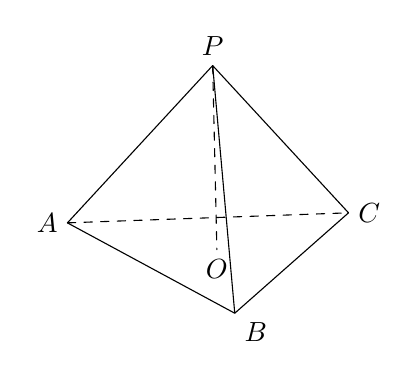
\begin{tikzpicture}[line cap=round,line join=round,scale=0.85]
  \coordinate (A) at (-2.15,0.20);
  \coordinate (B) at (0.35,-1.15);
  \coordinate (C) at (2.05,0.35);
  \coordinate (O) at (0.083,-0.20);
  \coordinate (P) at (0.02,2.55);

  % Hidden far edge and altitude in the source drawing.
  \draw[dashed] (A)--(C) (P)--(O);
  % Visible base edges and lateral edges.
  \draw (A)--(B)--(C) (P)--(A) (P)--(B) (P)--(C);

  \node[left] at (A) {$A$};
  \node[below right] at (B) {$B$};
  \node[right] at (C) {$C$};
  \node[below] at (O) {$O$};
  \node[above] at (P) {$P$};
\end{tikzpicture}
\end{center}
\nopagebreak[4]
\end{question}
\begin{question}
\gkti{20}某市 $2004$ 年底有住房面积 $1200\text{ \text{万平方米}}$，计划从 $2005$ 年起，每年拆除 $20\text{ \text{万平方米}}$ 的旧住房。假定该市每年新建住房面积是上年年底住房面积的 $5\%$。

（1） 分别求 $2005$ 年底和 $2006$ 年底的住房面积；

（2） 求 $2024$ 年底的住房面积。（计算结果以万平方米为单位，且精确到 $0.01$。）

\Needspace{0.4\textheight}
\end{question}
\begin{question}
\gkti{21}已知函数 $f(x)=x+\dfrac ax$ 的定义域为 $(0,+\infty)$，且 $f(2)=2+\dfrac{\sqrt2}{2}$。设点 $P$ 是函数图象上的任意一点，过点 $P$ 分别作直线 $y=x$ 和 $y$ 轴的垂线，垂足分别为 $M,N$。

（1） 求 $a$ 的值；

（2） 问：$\lvert PM\rvert\cdot\lvert PN\rvert$ 是否为定值？若是，则求出该定值；若不是，则说明理由；

（3） 设 $O$ 为坐标原点，求四边形 $OMPN$ 面积的最小值。
\nopagebreak[4]
\begin{center}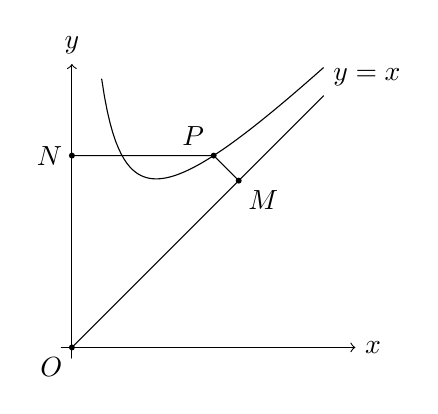
\begin{tikzpicture}[line cap=round,line join=round,scale=0.9]
  \coordinate (O) at (0,0);
  \coordinate (P) at (2.00,2.707107);
  \coordinate (N) at (0,2.707107);
  \coordinate (M) at (2.3535535,2.3535535);

  % Coordinate axes and the diagonal y=x.
  \draw[->] (0,-0.15)--(0,4.0) node[above] {$y$};
  \draw[->] (-0.15,0)--(4.0,0) node[right] {$x$};
  \draw (0,0)--(3.55,3.55) node[above right] {$y=x$};

  % Use the curve from the question after its given condition determines a=sqrt(2).
  % P is an illustrative sample point (x=2); the source gives no graph scale or coordinates.
  \draw plot[domain=0.42:3.55,samples=80,variable=\x] ({\x},{\x+sqrt(2)/\x});

  % Projection from P to the y-axis and to y=x.
  \draw (P)--(N) (P)--(M);

  \fill (O) circle (1.2pt);
  \fill (P) circle (1.2pt);
  \fill (M) circle (1.2pt);
  \fill (N) circle (1.2pt);
  \node[below left] at (O) {$O$};
  \node[above left] at (P) {$P$};
  \node[left] at (N) {$N$};
  \node[below right] at (M) {$M$};
\end{tikzpicture}
\end{center}
\nopagebreak[4]
\Needspace{0.4\textheight}
\end{question}
\begin{question}
\gkti{22}

（1） 求右焦点坐标是 $(2,0)$，且经过点 $(-2,-\sqrt2)$ 的椭圆的标准方程；

（2） 已知椭圆 $C$ 的方程是 $\dfrac{x^2}{a^2}+\dfrac{y^2}{b^2}=1\ (a>b>0)$。设斜率为 $k$ 的直线 $l$，交椭圆 $C$ 于 $A,B$ 两点，$AB$ 的中点为 $M$。证明：当直线 $l$ 平行移动时，动点 $M$ 在一条过原点的定直线上；

（3） 利用（2）所揭示的椭圆几何性质，用作图方法找出下面给定椭圆的中心，简要写出作图步骤，并在图中标出椭圆的中心。
\nopagebreak[4]
\begin{center}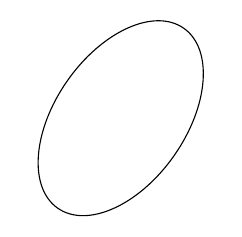
\begin{tikzpicture}[line cap=round,line join=round,scale=0.9]
  % The source shows only an unlabelled tilted ellipse; no axes or center mark.
  \draw[rotate=55] (0,0) ellipse (1.55 and 0.92);
\end{tikzpicture}
\end{center}
\nopagebreak[4]

\end{question}